\section{Software in the Loop}

\subsection{Monte-Carlo}

The Monte-Carlo method runs repeated simulations with random variations of parameters.
In this case, the Monte-Carlo method is used to determine the robustness and sensitivity of the closed-loop system (Rocket, Estimator, Controller) to modelling uncertainty and external disturbances.
The Monte-Carlo method is used as the simulation is non-linear and has multiple uncertain parameters, such as sensor noise and bias, wind disturbances, actual aerodynamic behaviour, and more. 

In Matlab/Simulink, multiple simulations can be run using the \texttt{parsim} function, which supports sweeping of parameters.
The computations can be offloaded to a compute server with the \texttt{batchsim} function.

In the flight simulation framework, some parameters are already randomly varied for each simulation, such as the sensor biases.
Other parameters are explicitly swept between lower and upper limits for the Monte-Carlo simulations, these are listed in \autoref{tab:monte-carlo-params}. 
Some parameters are varied for an absolute value (e.g. wind speed), while others are a factor of the nominal value (e.g. engine thrust).

\begin{table}[ht]
    \centering
    \begin{tabularx}{\linewidth}{l c c c c X }
         Parameter & Nom. & $>$ & $<$ & Unit & Reason \\[0.2em]
         \hline \\[-1em]
         Engine &&&&& \\
         thrust & 1 & 0.85 & 1.05 & $\cdot$ & Performance variations $\to$ velocity and apogee \\
         %\hline \\[-1em]
         Wind \\ const. speed & 0 & 0 & 20 & m/s & Weather variations, causes pitch over \\
         gust speed & 0 & 0 & 30 & m/s  & Weather, test velocity and coefficient estimate \\
         %\hline \\[-1em]
         Canard \\ coefficient & 1 & $-1$ & $2$ & $\cdot$ & Roll reversal, test coefficient estimation \\
         backlash & 0 & 0 & 1 & deg & Gearing uncertainty, test coefficient and angle estimation, test controller tracking \\
         cant angle & 0 & 0 & 0.5 & deg & Actuator misalignment variations, test spin up during boost and controller tracking
    \end{tabularx}
    \caption{Sweep parameters for Monte-Carlo simulations}
    \label{tab:monte-carlo-params}
\end{table}

\begin{figure}[ht]
    \centering
    \begin{subfigure}{\textwidth}
        \centering
        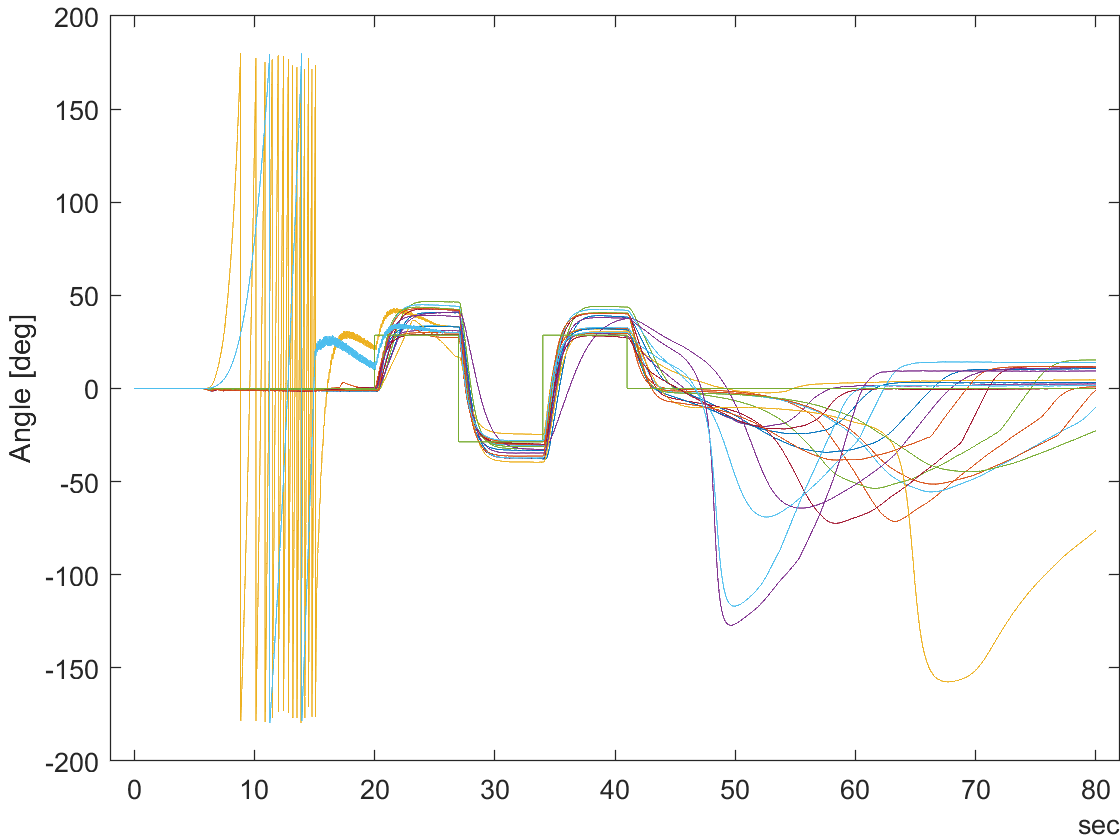
\includegraphics[width=0.4\textwidth]{images-results/controller_simulation_20250715_batch_all_1.png}
        \caption{Controller roll angle}
        \label{fig:result_mc_all_1_control}
    \end{subfigure}
    \begin{subfigure}{\textwidth}
        \centering
        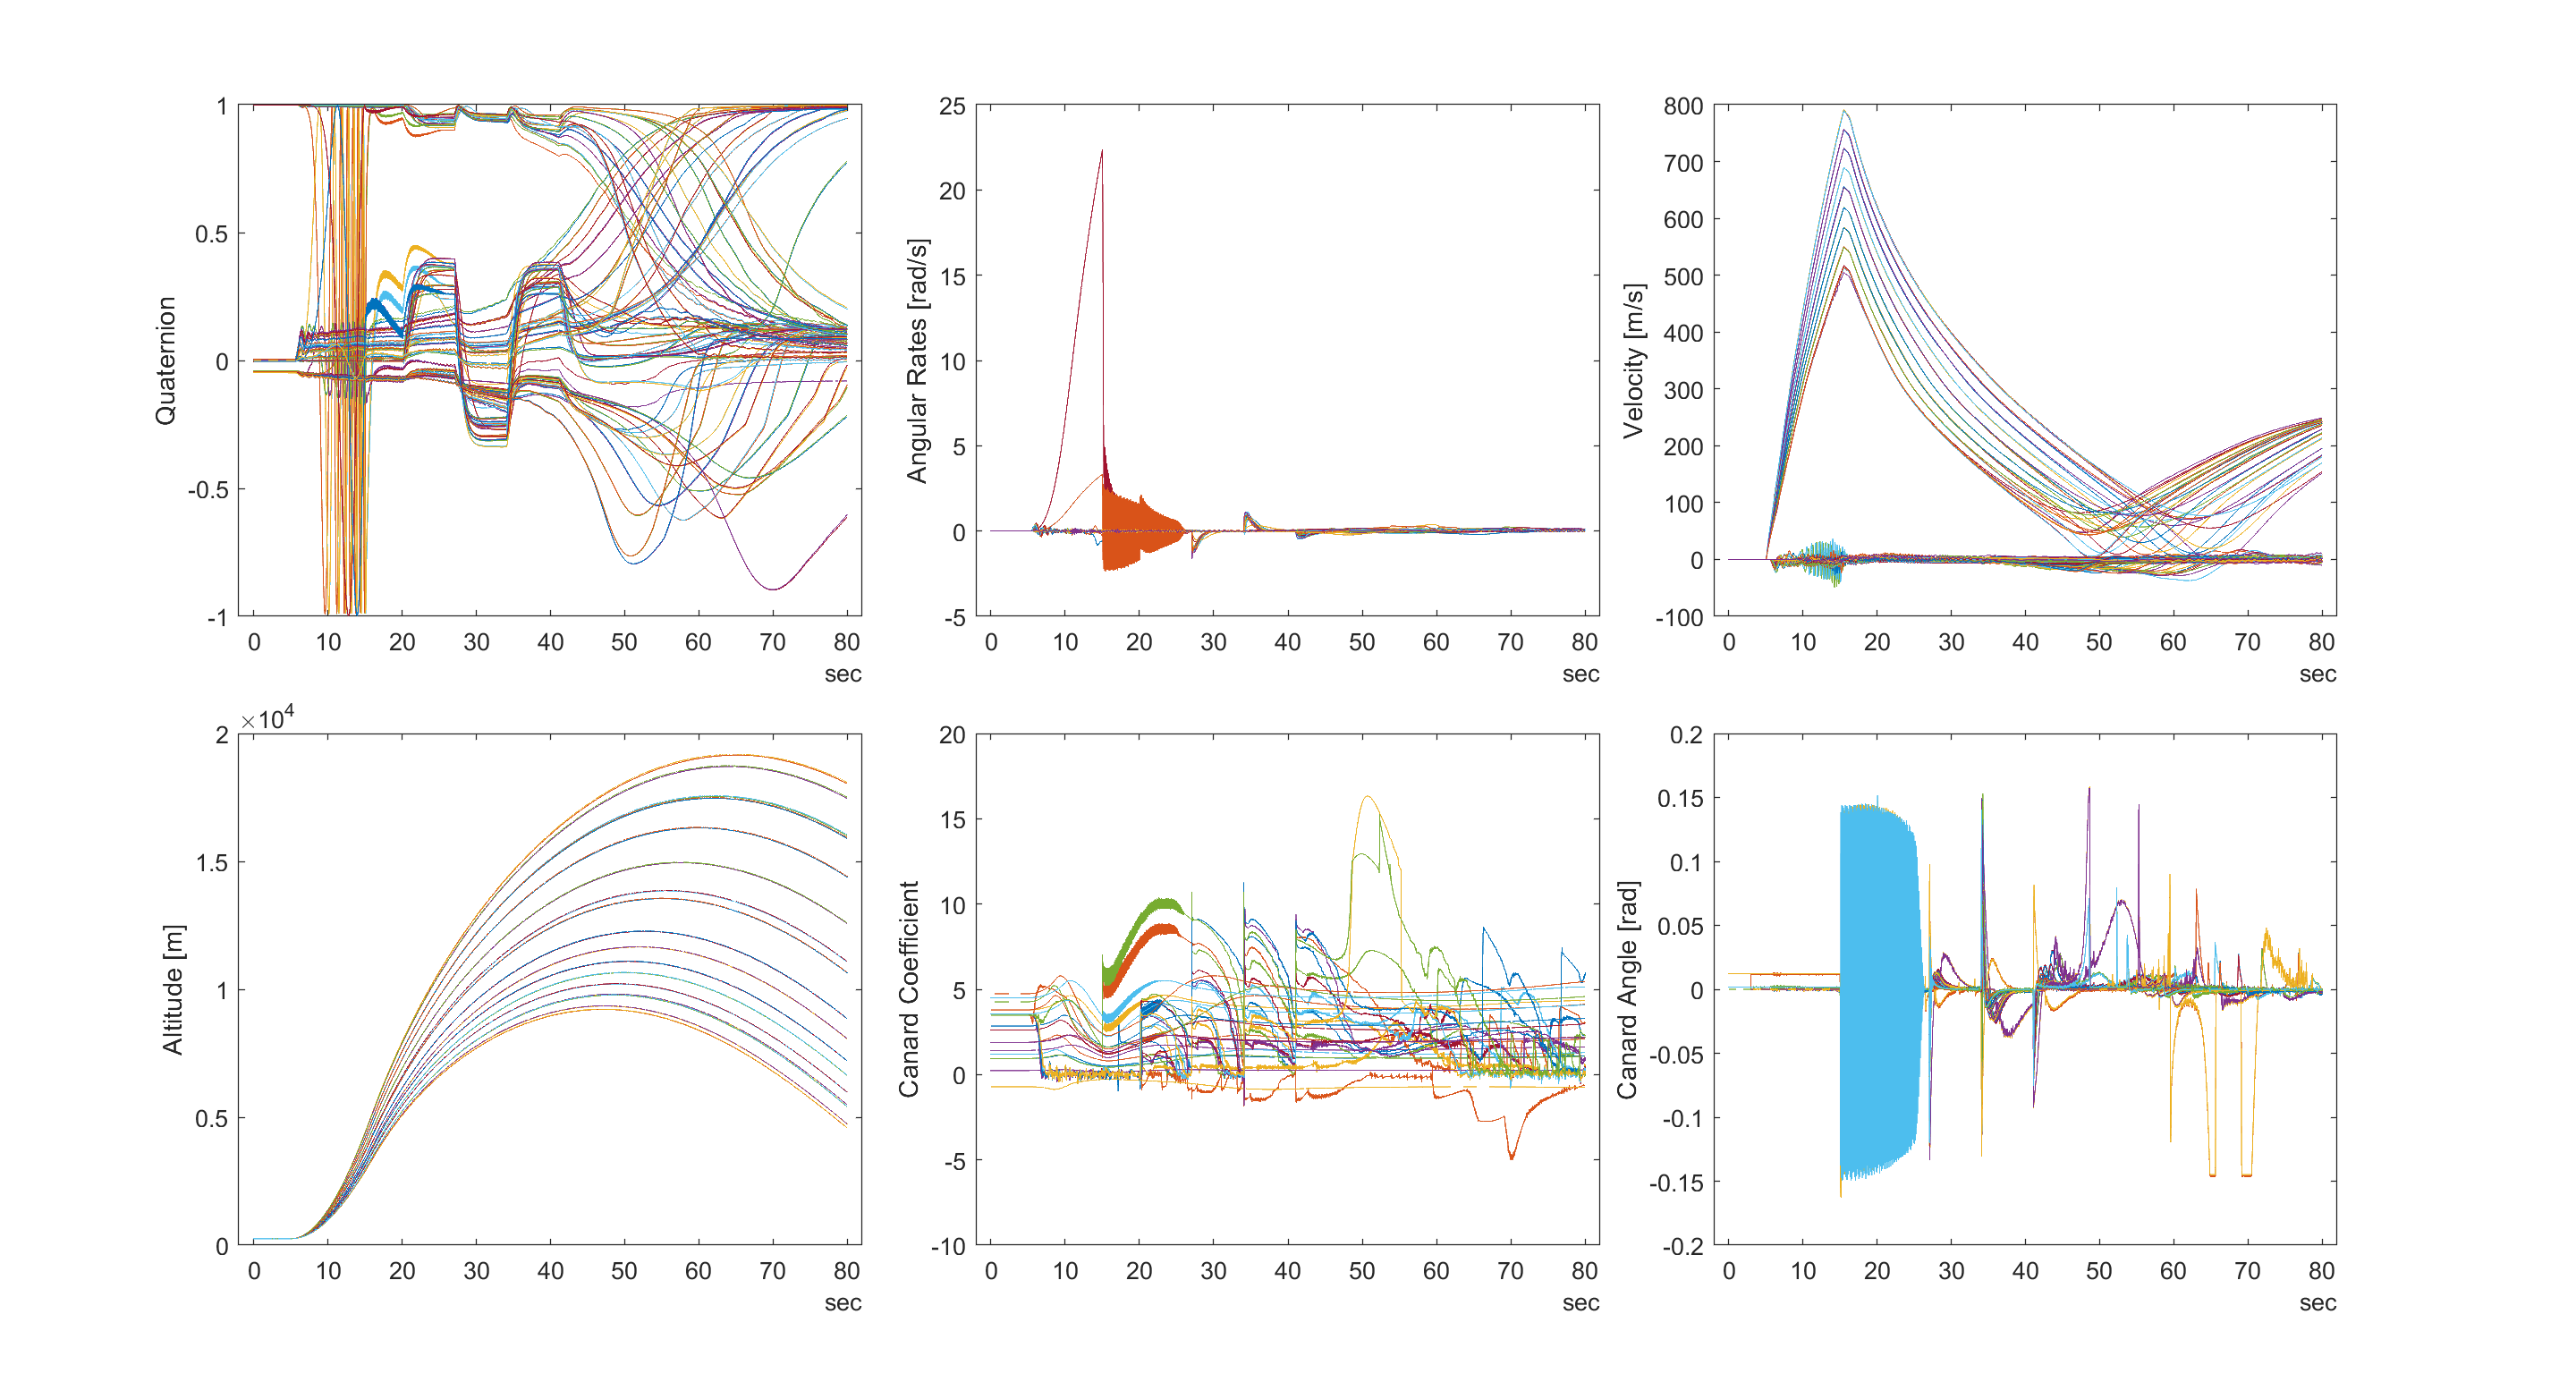
\includegraphics[width=0.95\textwidth]{images-results/estimator-simulation_20250715_batch_all_1.png}
        \caption{Estimator}
        \label{fig:result_mc_all_1_est}
    \end{subfigure}
    \begin{subfigure}{\textwidth}
        \centering
        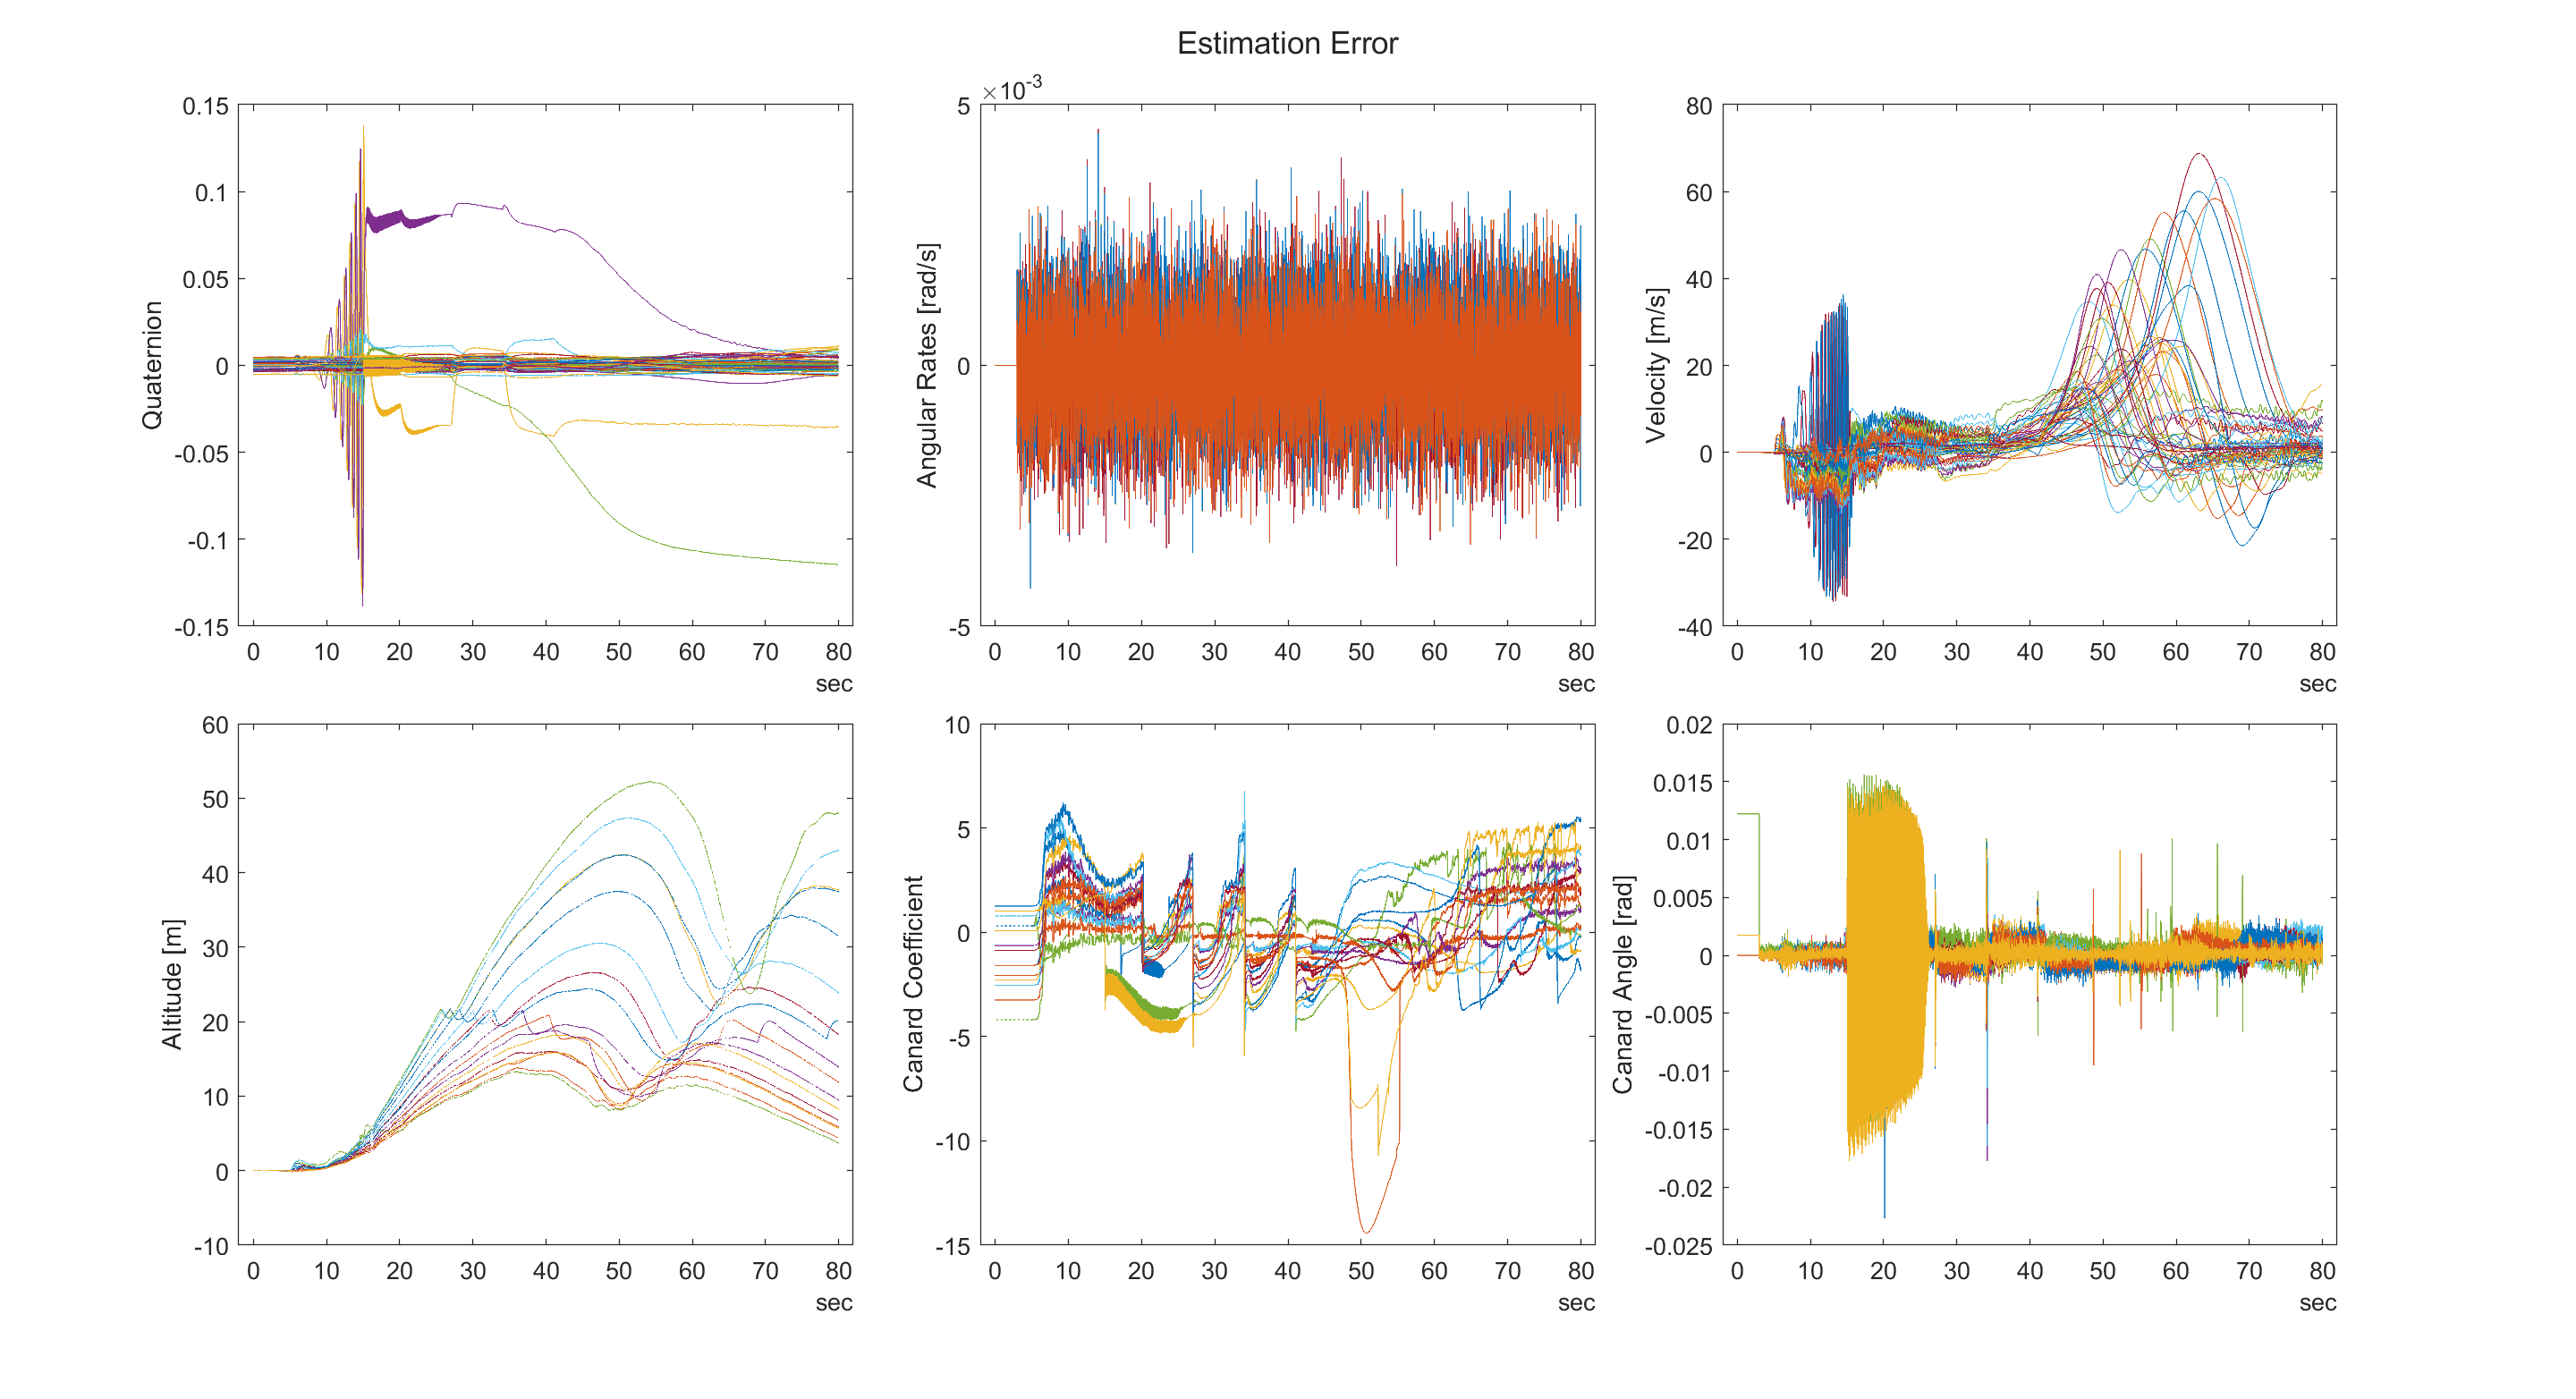
\includegraphics[width=0.95\textwidth]{images-results/estimator-simulation_20250715_batch_all_1_error.png}
        \caption{Estimation error}
        \label{fig:result_mc_all_1_error}
    \end{subfigure}
    \caption{Monte-Carlo simulation run varying all parameters}
    \label{fig:result_mc_all_1}
\end{figure}

\begin{figure}[ht]
    \centering
    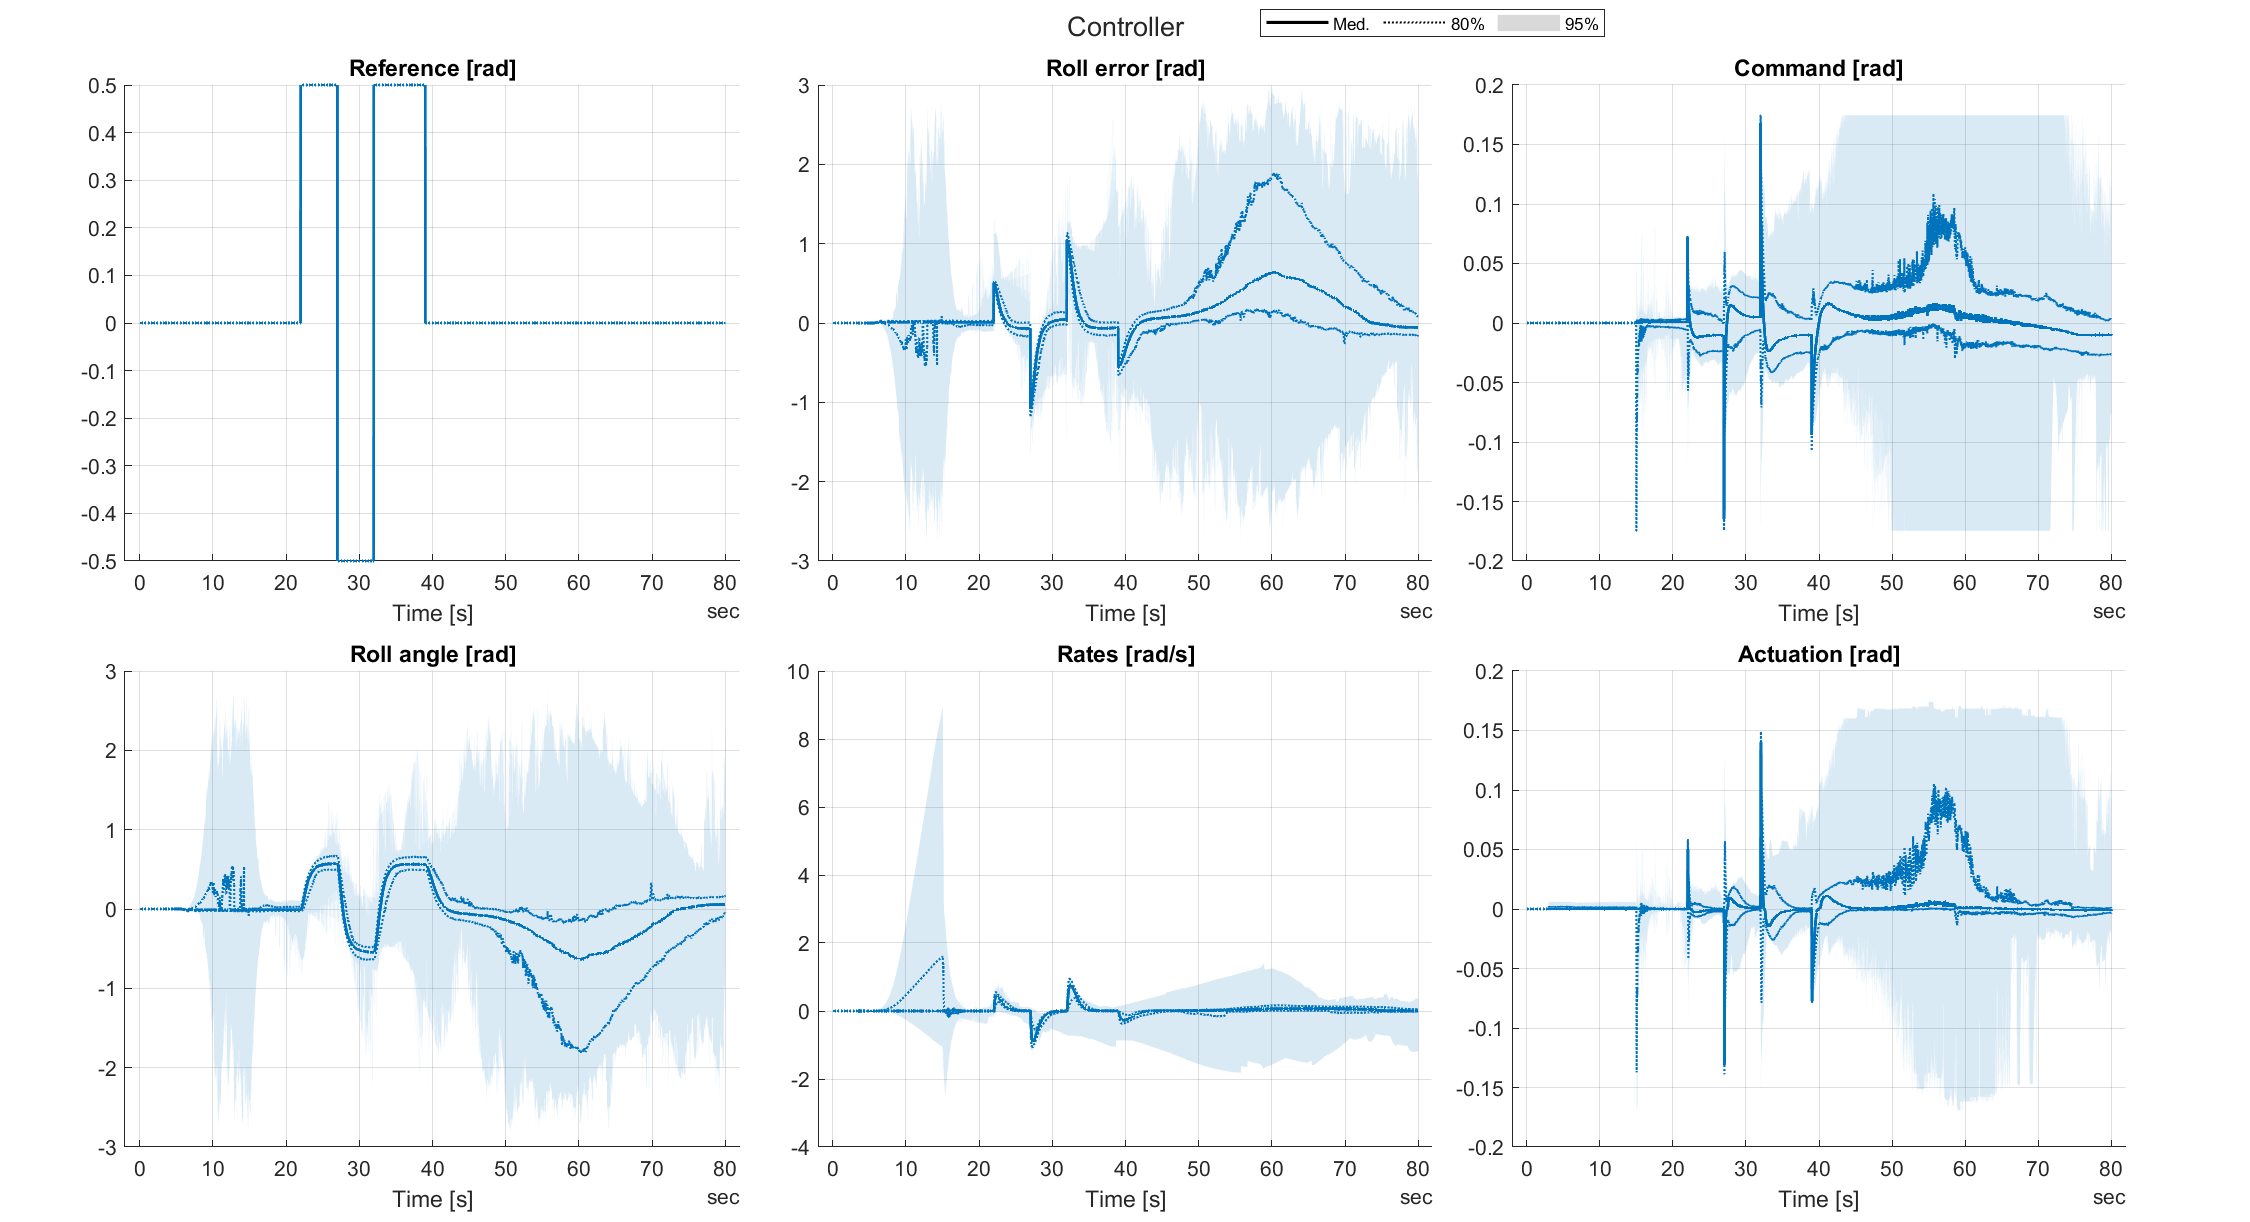
\includegraphics[width=\linewidth]{images-results/result_stats_control_fixaccel_300.png}
    \caption{Statistics of controller variables for Monte-Carlo with 300 simulations}
    \label{fig:results_mc_stat_control}
\end{figure}
\begin{figure}[ht]
    \centering
    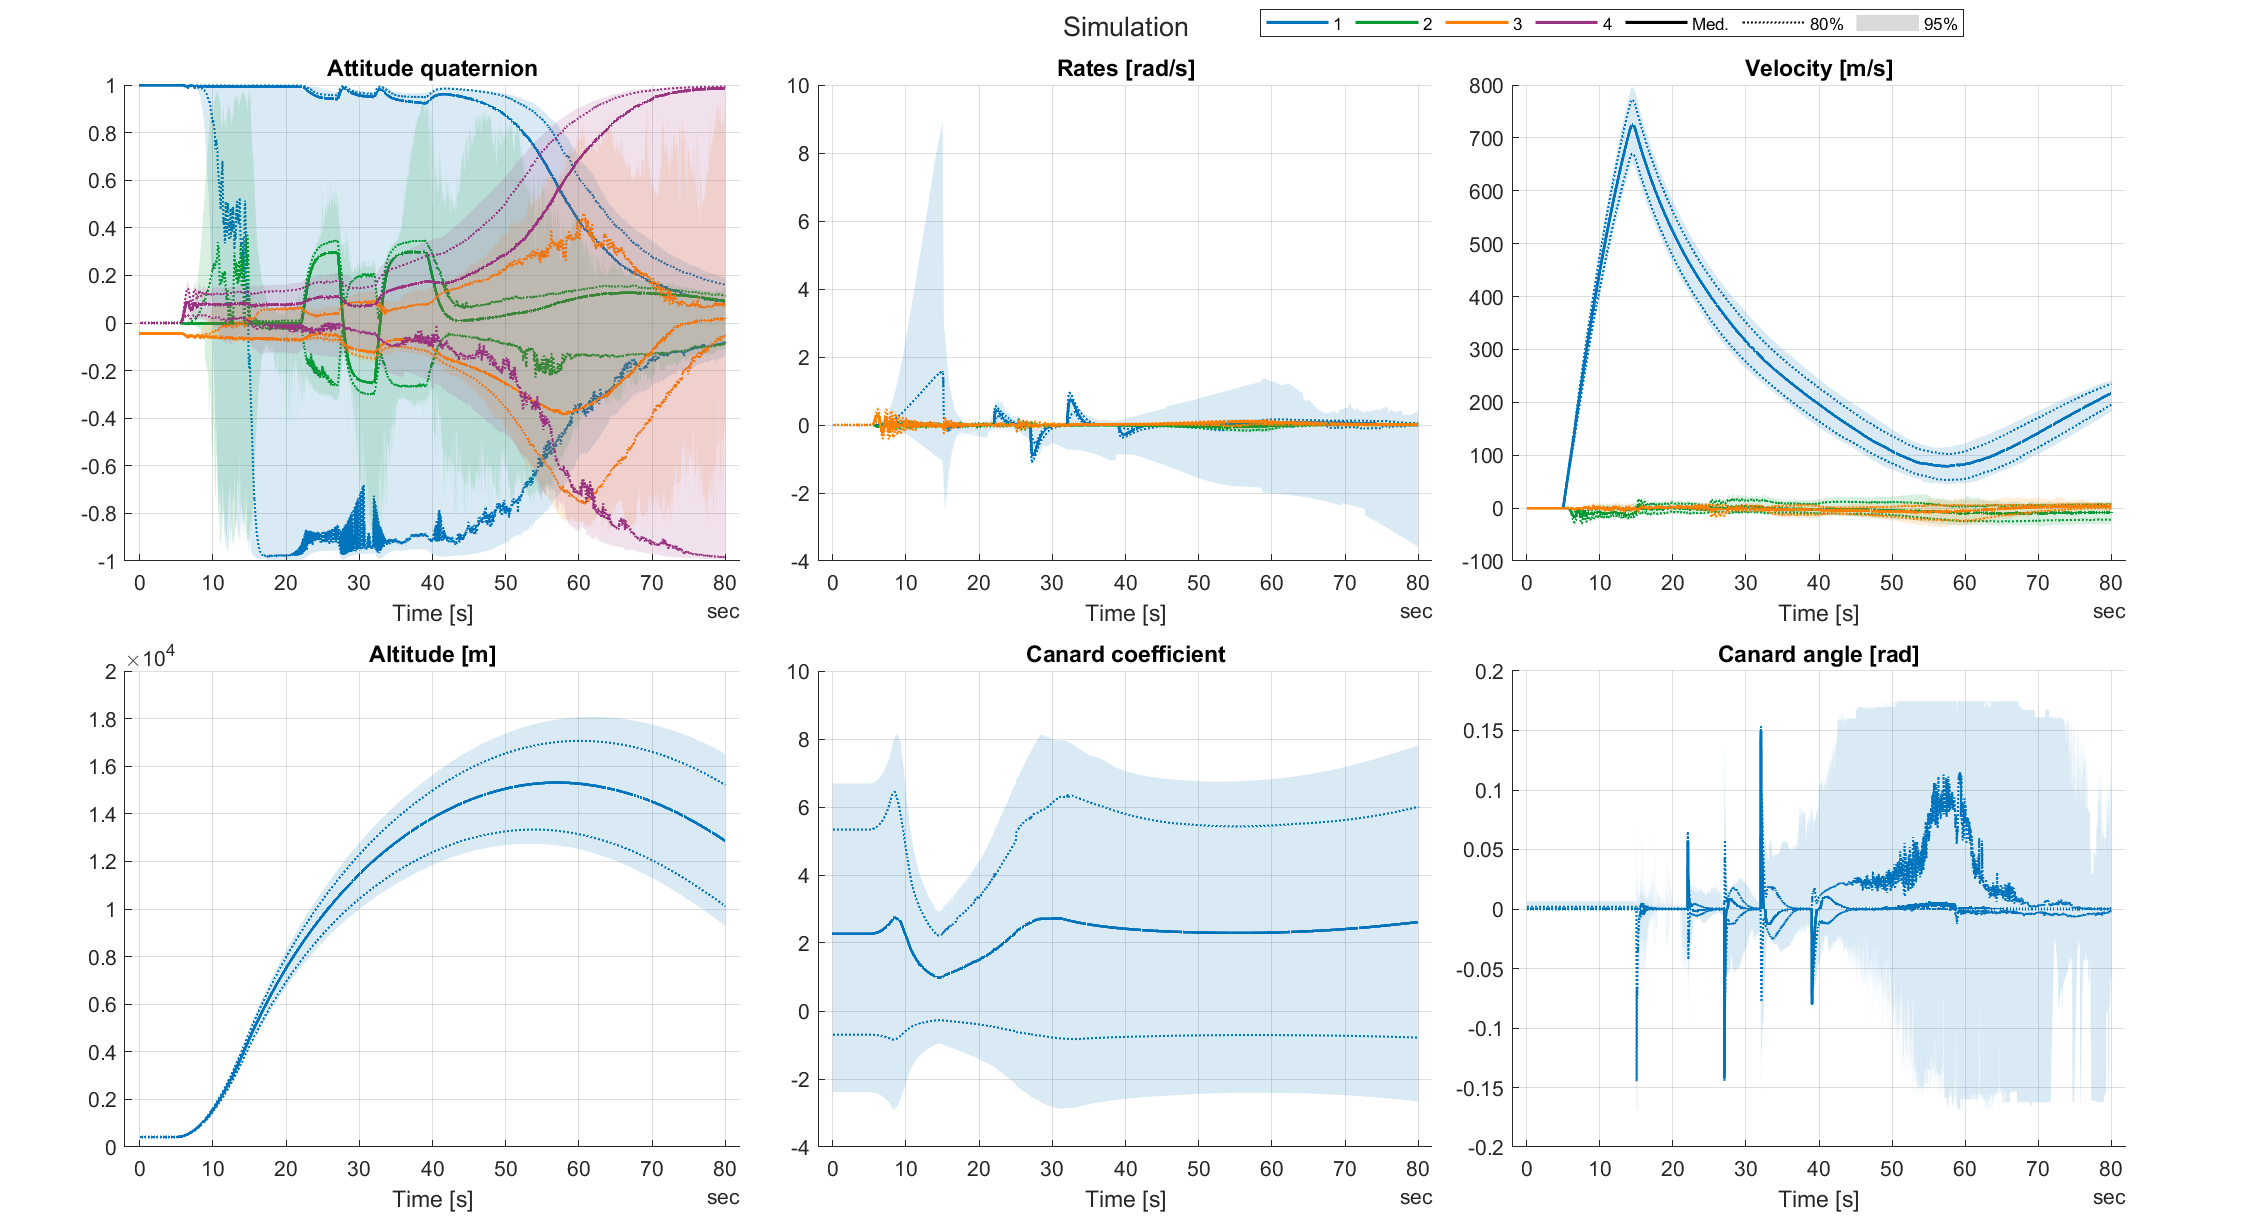
\includegraphics[width=\linewidth]{images-results/result_stats_sim_fixaccel_300.png}
    \caption{Statistics of simulation state for Monte-Carlo with 300 simulations}
    \label{fig:results_mc_stat_sim}
\end{figure}
\begin{figure}[ht]
    \centering
    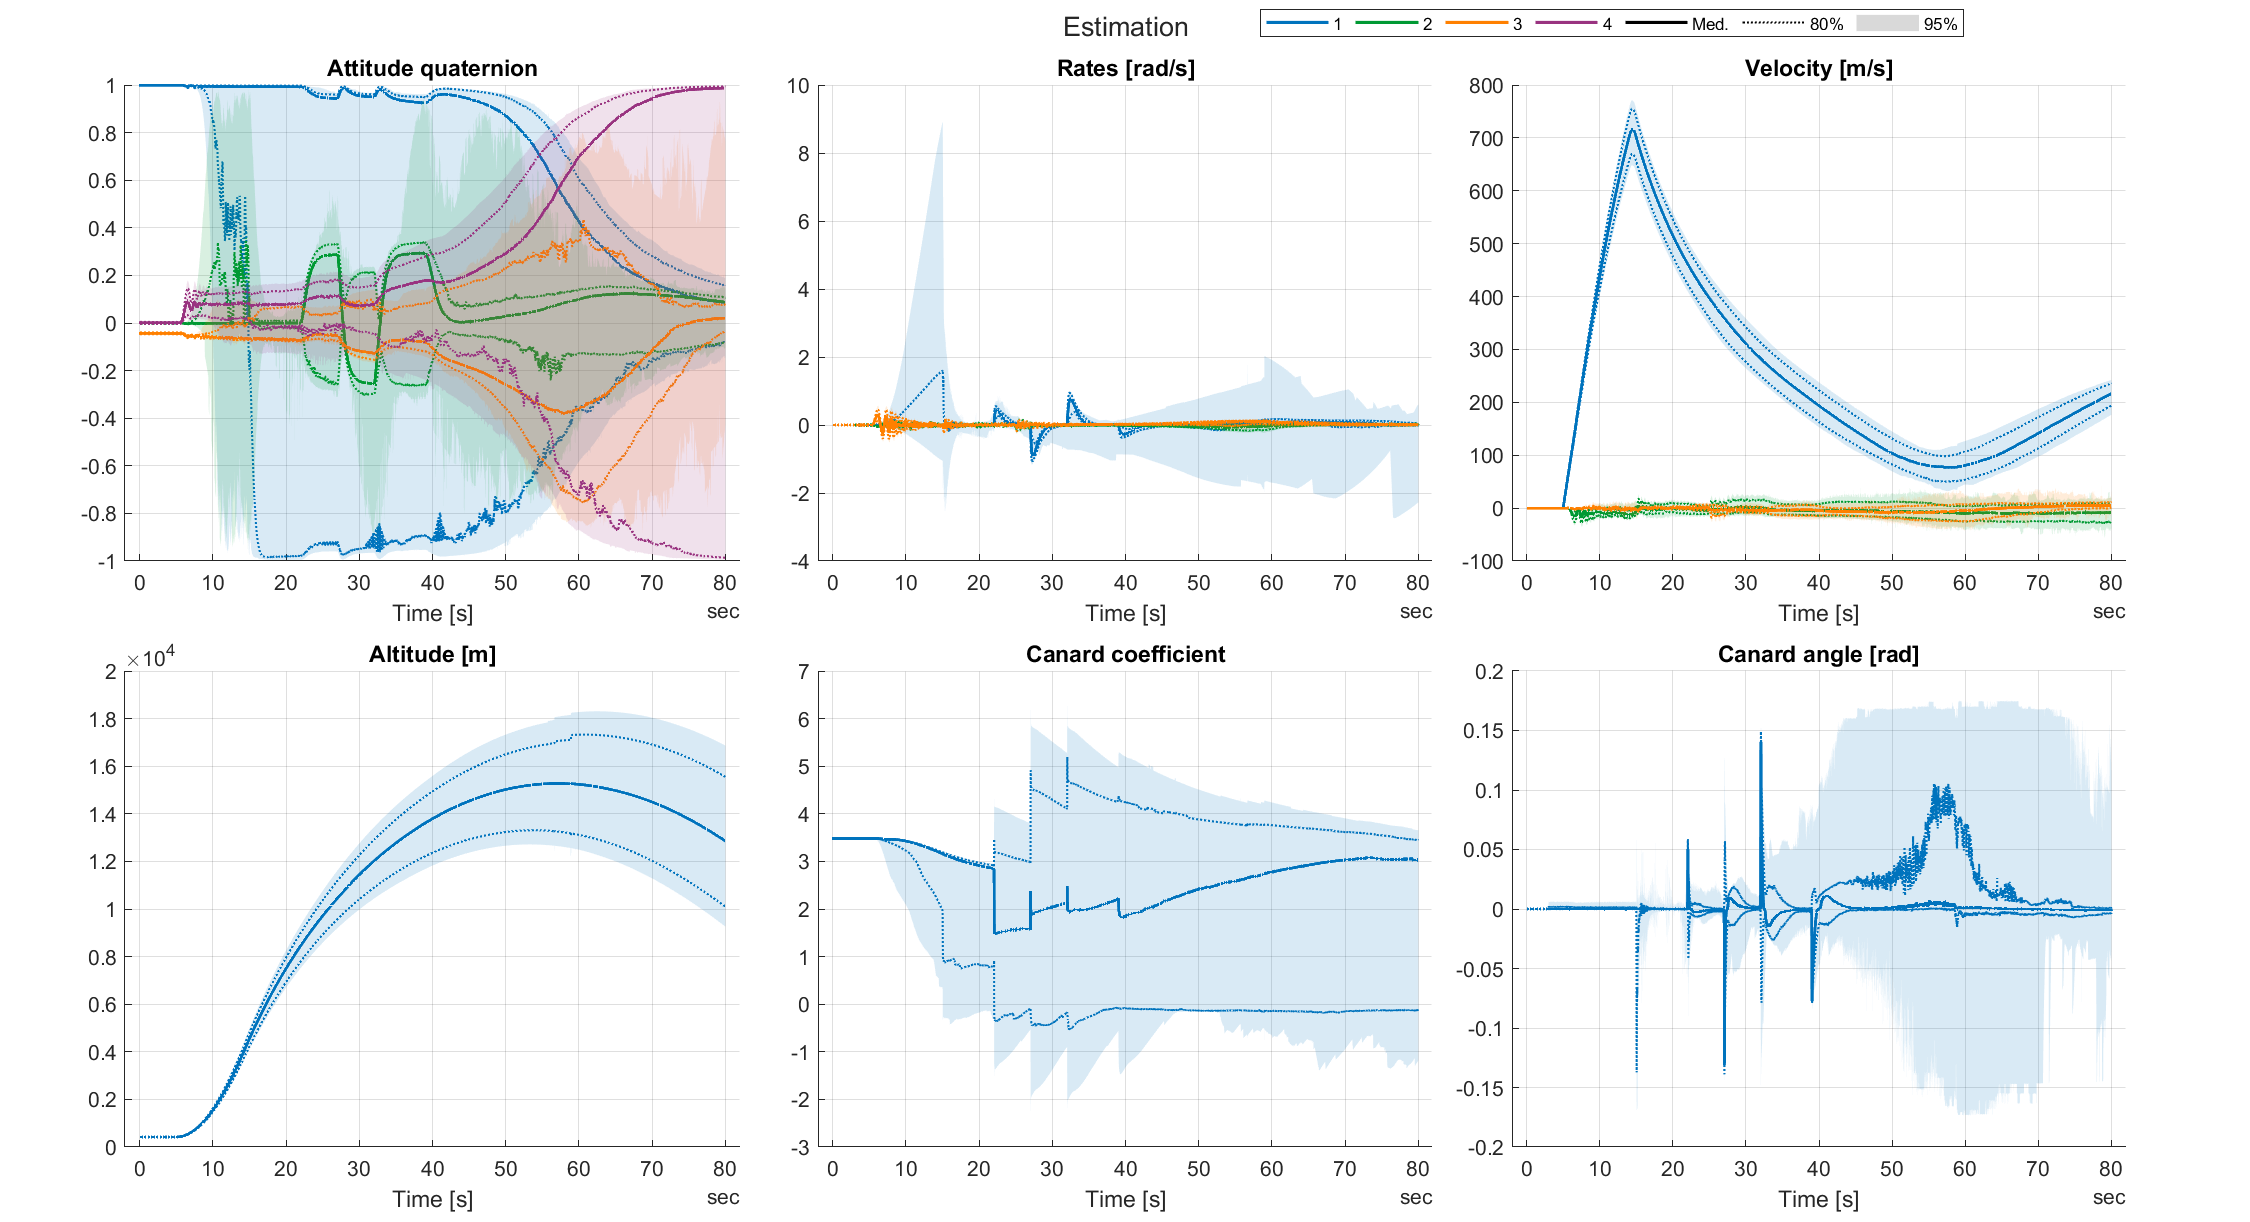
\includegraphics[width=\linewidth]{images-results/result_stats_est_fixaccel_300.png}
    \caption{Statistics of estimated state for Monte-Carlo with 300 simulations}
    \label{fig:results_mc_stat_est}
\end{figure}
\begin{figure}[ht]
    \centering
    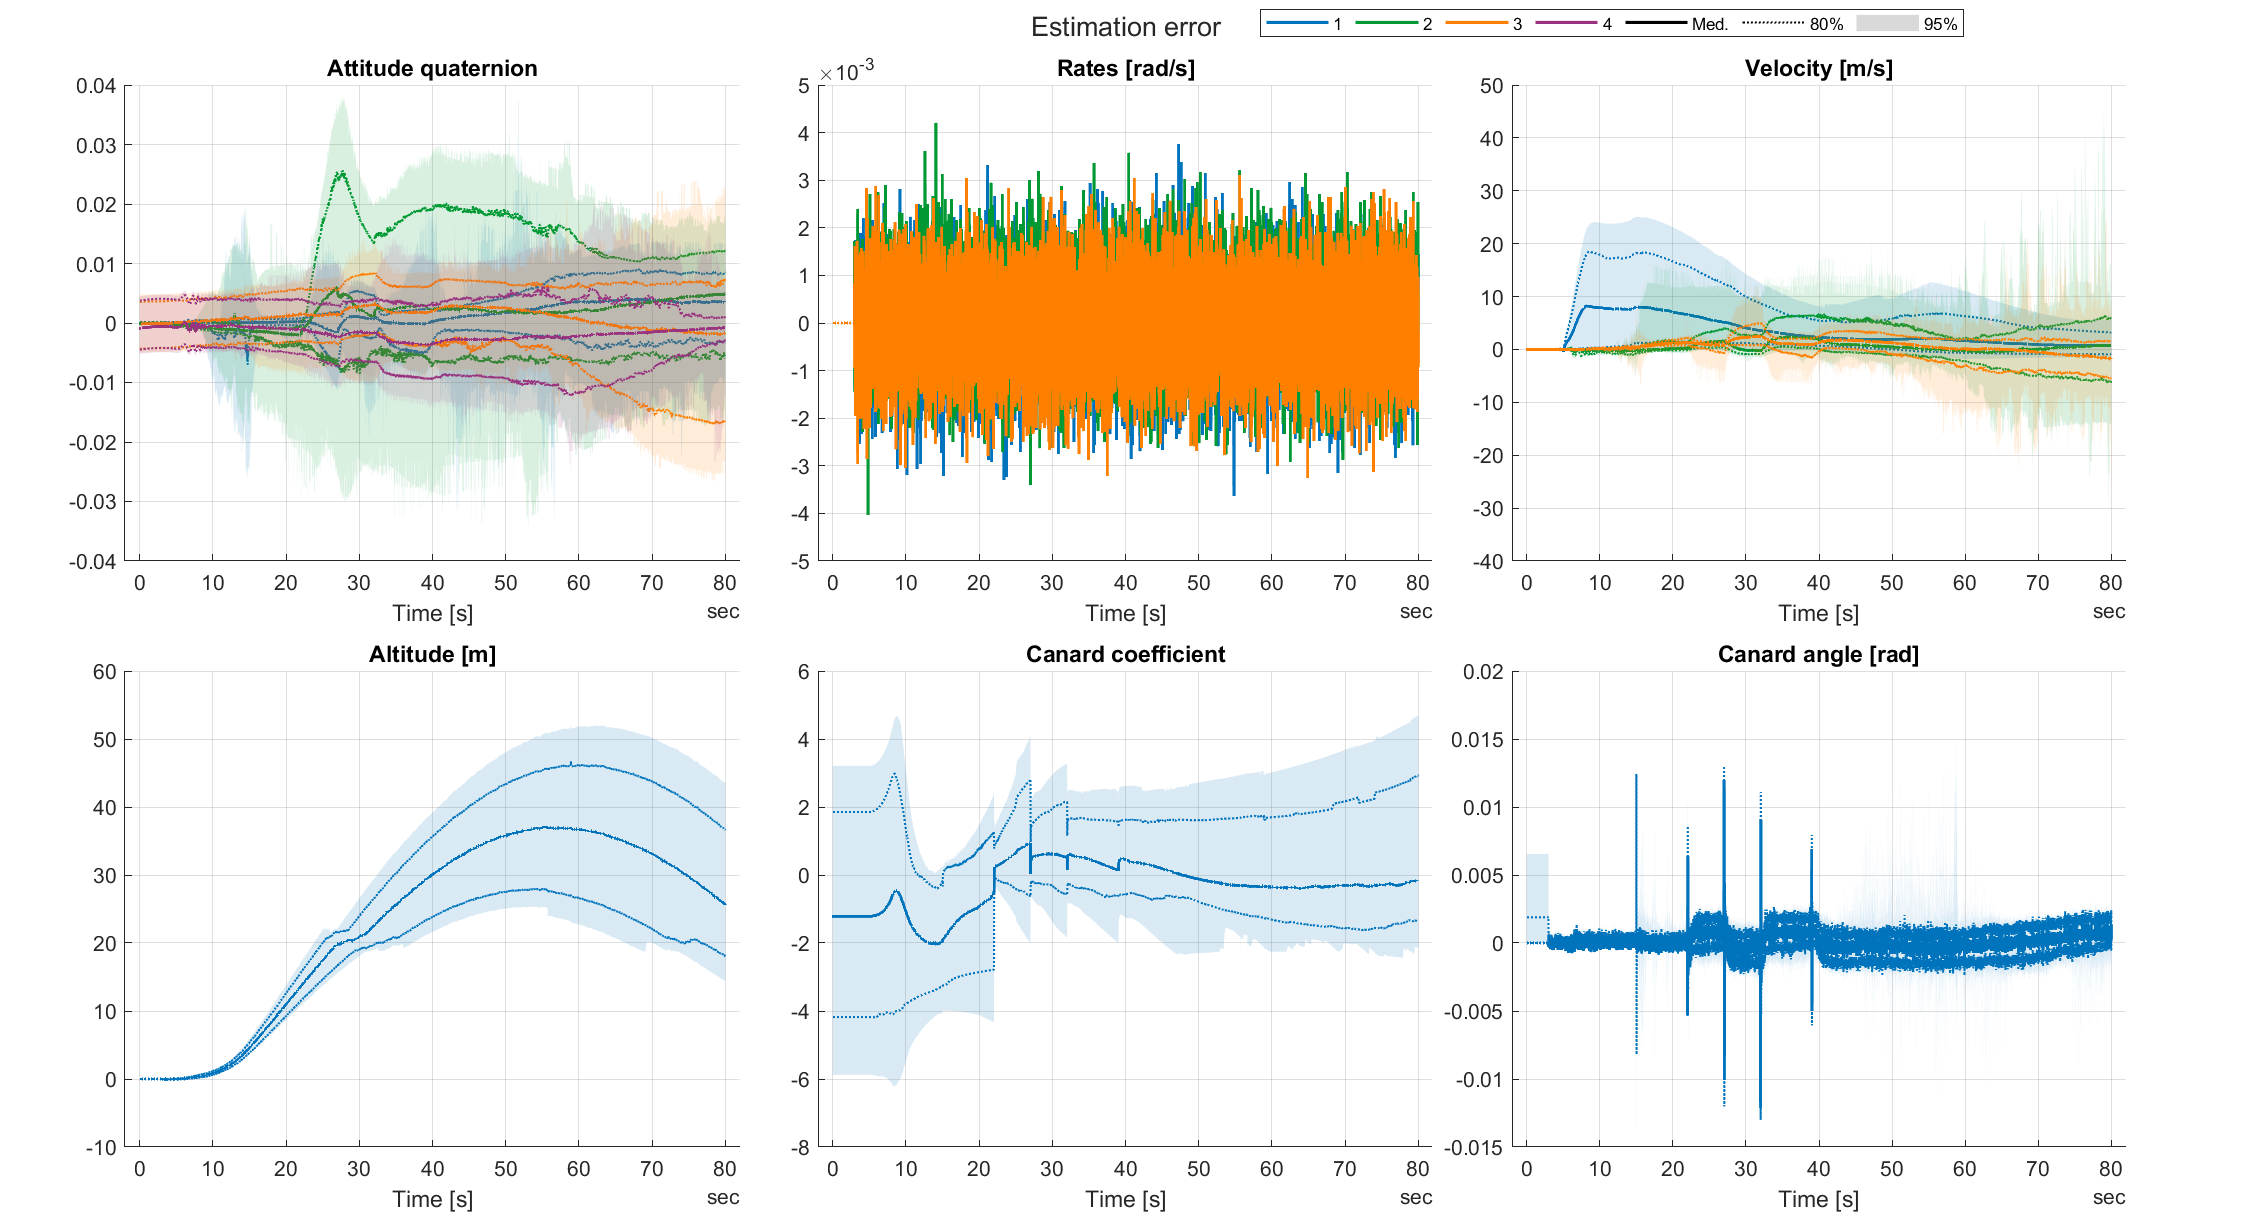
\includegraphics[width=\linewidth]{images-results/result_stats_error_fixaccel_300.png}
    \caption{Statistics of estimation error for Monte-Carlo with 300 simulations}
    \label{fig:results_mc_stat_error}
\end{figure}
\begin{figure}[ht]
    \centering
    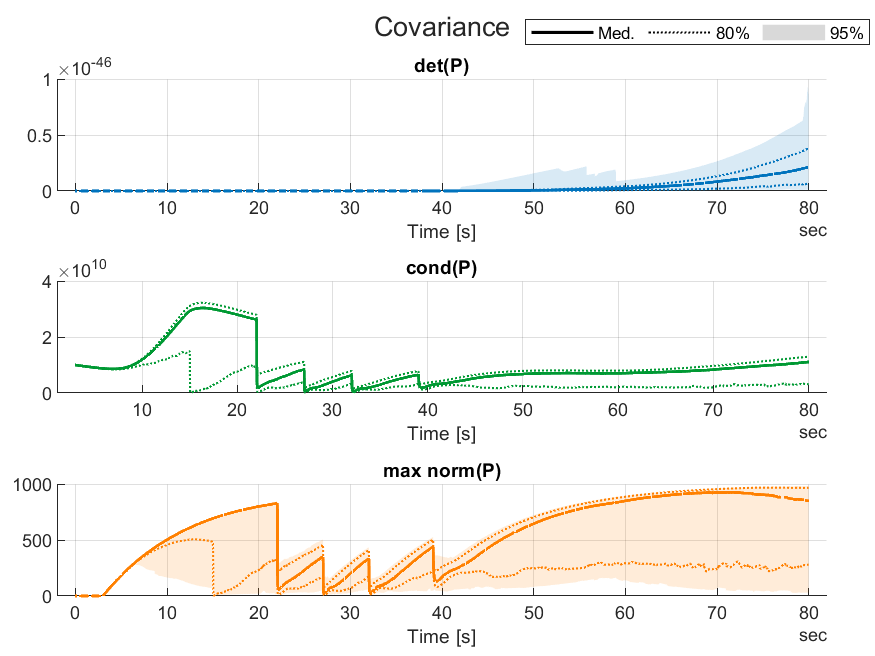
\includegraphics[width=0.65\linewidth]{images-results/result_stats_cov_fixaccel_300.png}
    \caption{Statistics of covariance matrix for Monte-Carlo with 300 simulations}
    \label{fig:results_mc_stat_cov}
\end{figure}



\section{Hardware in the Loop}

\clearpage
\section{Testflight}
The Testflight launch was conducted on May 10th 2025 near Louisville, Kentucky.
The resulting state estimation data is shown in \autoref{fig:testflight}.

Due to an error with internal logging only the telemetry data is available. This data was transmitted by the Processor Board to the rocket CAN bus, sent over radio telemetry, and logged by the ground station computer.
Due to the telemetry bandwidth and lossy connection, data points are not recorded at high speeds and regular intervals, and in some cases bits were dropped resulting in larger jumps of the data (e.g. at about $t=8\mathrm{s}$, the altitude jumps from 250m to 512m instead of 256m).   

Due to a safety lockout triggered by a timer, the canard was commanded to zero for the entirety of the flight.
Therefore the rocket had no control authority, and some misalignment of the canards and fin cant led to a slow roll rate with a peak of about 2 rad/s, as can be seen in \autoref{fig:testflight-w}.

The rocket lifts off at about $t=8\mathrm{s}$, and reaches apogee at about $t=28\mathrm{s}$.
At $t=31\mathrm{s}$ the recovery system is deployed, at which point the mission of the Controls subsystem ends. 
After recovery deployment the state estimation becomes unreliable, as descent under parachutes is not modelled.

Overall the Estimator performed well, as simulations line up with actual flight. 

\begin{figure}[ht]
    \centering   
    \begin{subfigure}{0.49\textwidth}
        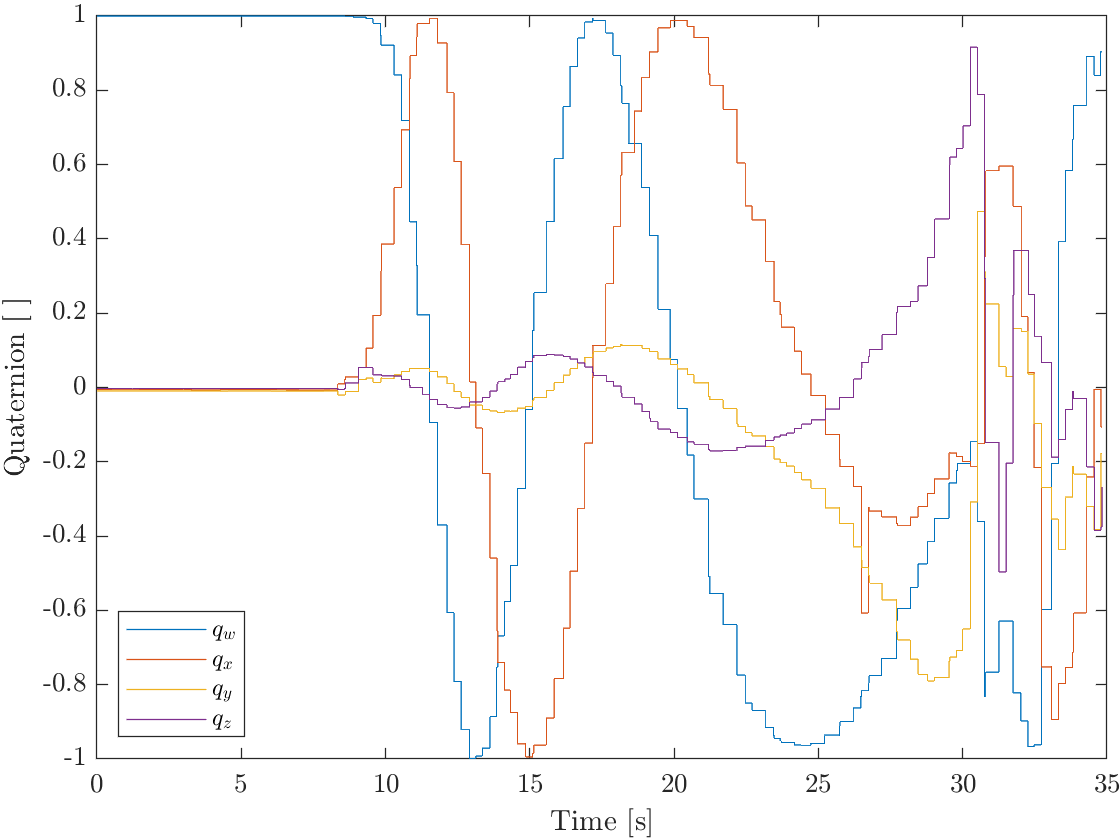
\includegraphics[width=0.95\textwidth]{images-results/testflight_q.png}
        \caption{Attitude Quaternion}
        \label{fig:testflight-q}
    \end{subfigure}
    \begin{subfigure}{0.49\textwidth}
        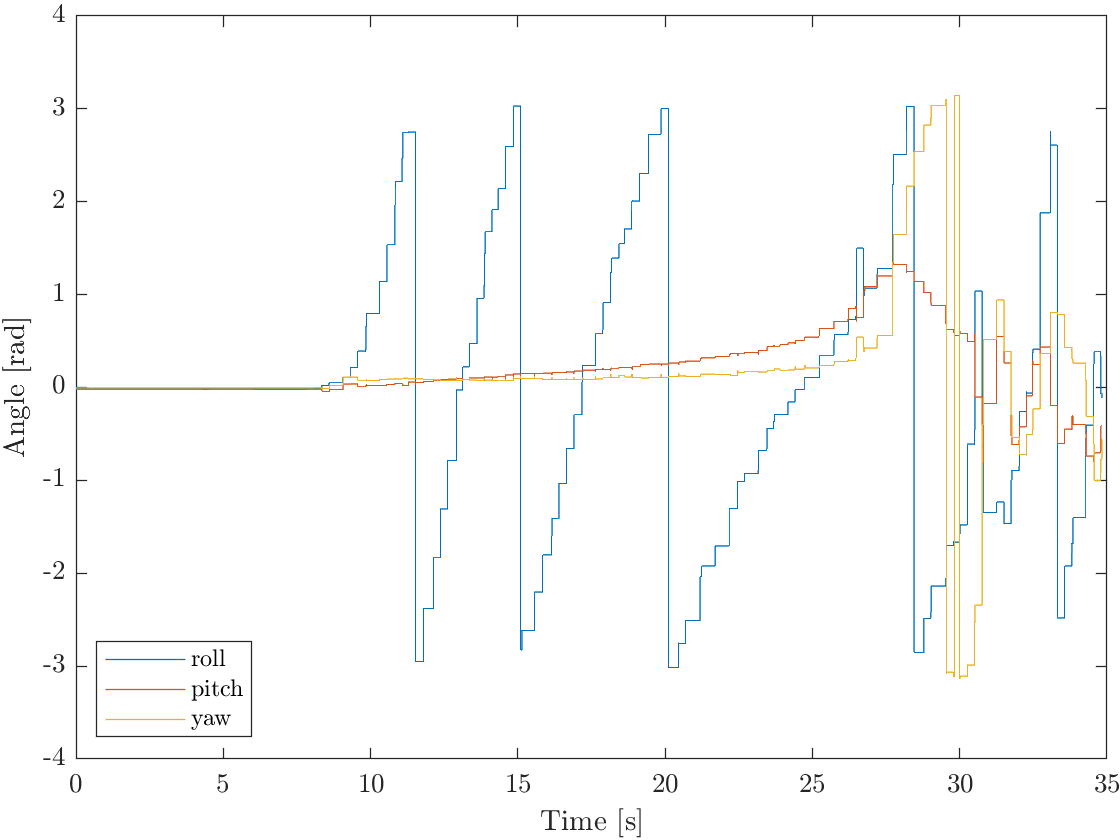
\includegraphics[width=0.95\textwidth]{images-results/testflight_euler.png}
        \caption{Attitude Euler angles}
        \label{fig:testflight-euler}
    \end{subfigure}
    \begin{subfigure}{0.49\textwidth}
        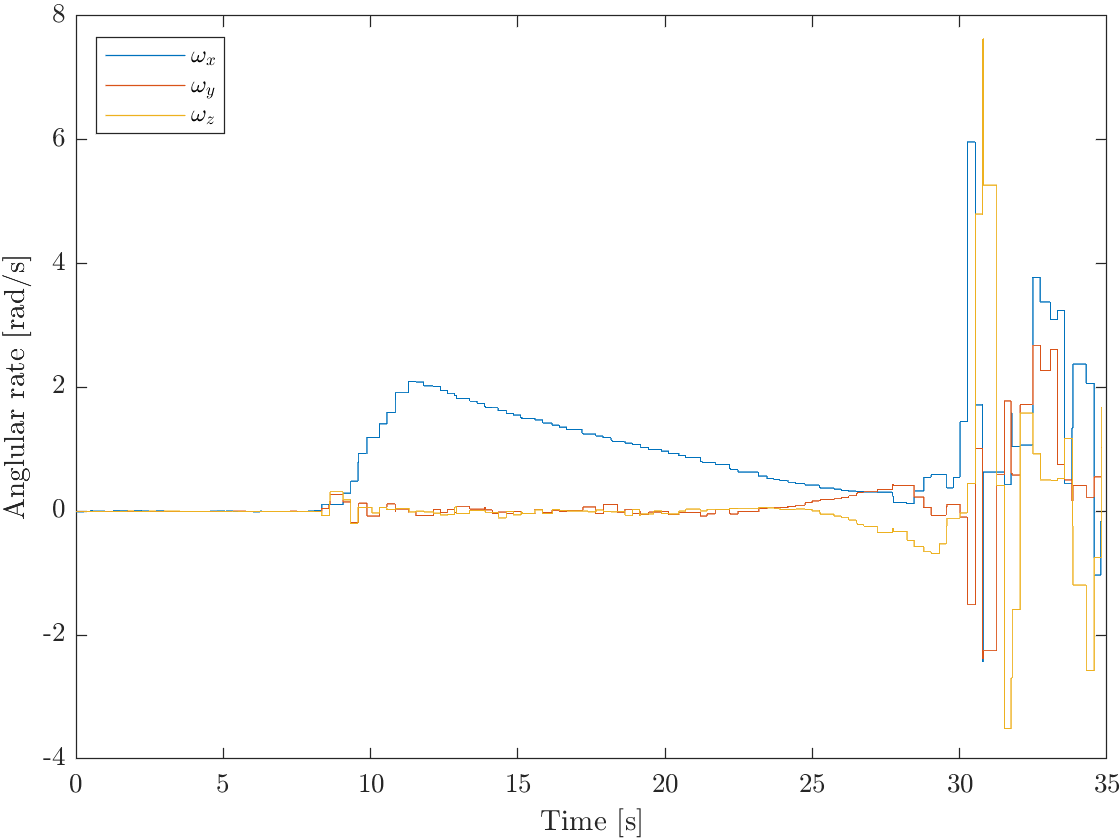
\includegraphics[width=0.95\textwidth]{images-results/testflight_w.png}
        \caption{Angular rates}
        \label{fig:testflight-w}
    \end{subfigure}
    \begin{subfigure}{0.49\textwidth}
        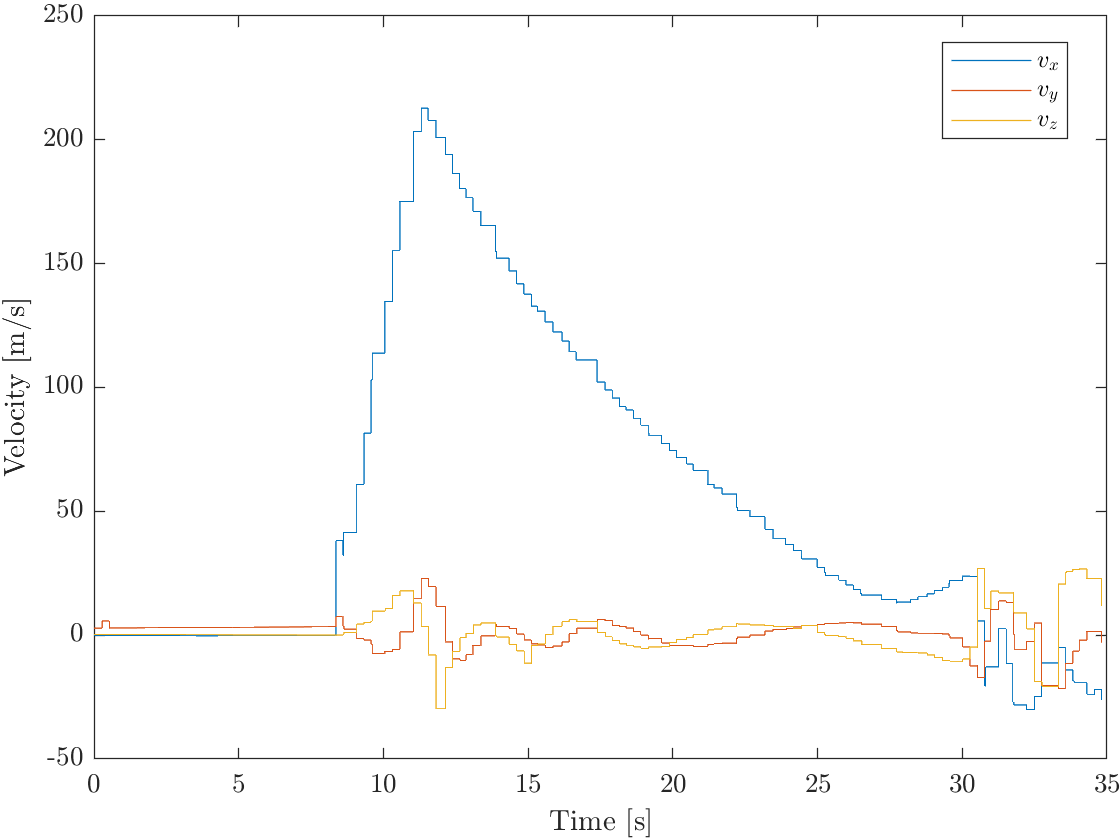
\includegraphics[width=0.95\textwidth]{images-results/testflight_v.png}
        \caption{Body velocity}
        \label{fig:testflight-v}
    \end{subfigure}
    \begin{subfigure}{0.49\textwidth}
        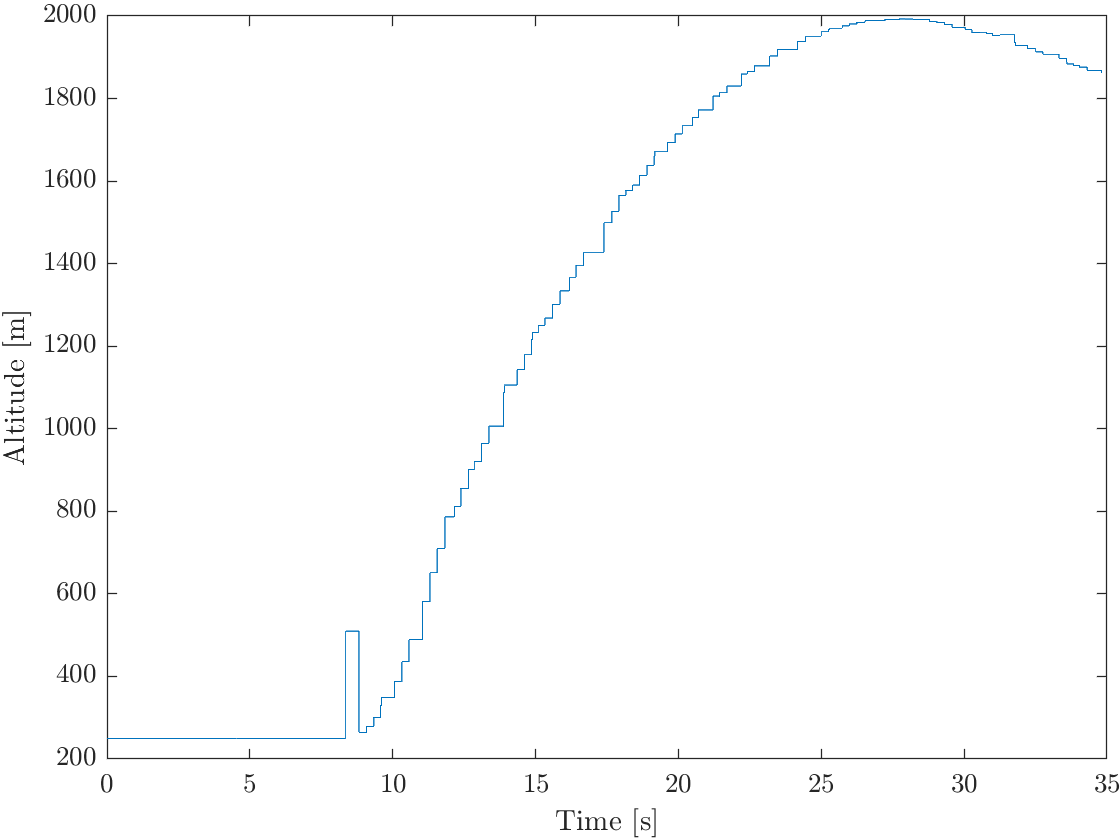
\includegraphics[width=0.95\textwidth]{images-results/testflight_alt.png}
        \caption{Altitude}
        \label{fig:testflight-alt}
    \end{subfigure}
    \begin{subfigure}{0.49\textwidth}
        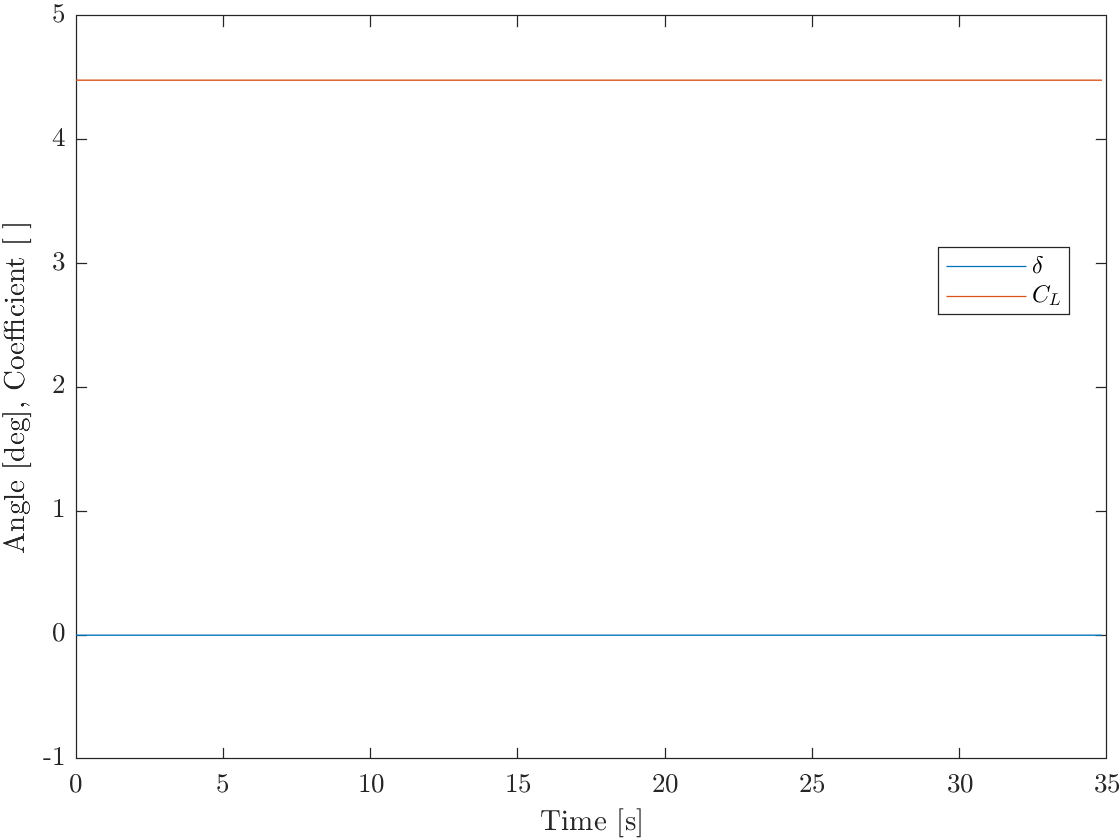
\includegraphics[width=0.95\textwidth]{images-results/testflight_canard.png}
        \caption{Canard}
        \label{fig:testflight-canard}
    \end{subfigure}
    \caption{Testflight telemetry, estimated state}
    \label{fig:testflight}
\end{figure}

\clearpage
\section{Competition flight}
